\documentclass[12pt]{article}

%===============================
%
%          📦 Paquetes
%
%===============================

\usepackage[a4paper, top=3cm, bottom=3cm, left=3cm, right=3cm]{geometry}
\usepackage[spanish]{babel}
\usepackage[utf8]{inputenc}
\usepackage{amsmath}
\usepackage{multicol}
\usepackage{graphicx}
\usepackage{hyperref}
\usepackage{booktabs}
\usepackage{pgfplots}
\pgfplotsset{compat=1.18}

\title{
  \vspace{2cm}
  \pagenumbering{gobble}
  
\includegraphics[width=5cm]{./assets/logo-utp.png} \\
  \vspace{1cm}
  \textbf{Universidad Tecnológica del Perú} \\
  \vspace{2cm}
  \textbf{Gestión de Riesgos} \\
  \vspace{1cm}
  \large \textbf{Avance de Informe}
}
\author{
  \textbf{Torres Vara, Mateo Nicolas} - \texttt{U24308542} \\
  \texttt{Sección 32554}
}



\begin{document}
\maketitle
\begin{center}

  Docente: Elvis Henry Guzman Aquije

\end{center}

%======================================
%
%          📚 Inicio del documento
%
%======================================

\newpage
\section*{Análisis de Macroentorno}

\subsection*{Oportunidades}
\begin{itemize}
  \item Creciente demanda en el Perú por carreras técnicas de corta duración y rápida inserción laboral.
  \item Expansión de la digitalización y transformación digital en empresas (mayor demanda en TI, software, data).
  \item Alianzas con empresas globales (IBM, AWS, Cisco, Huawei, Oracle) que refuerzan la empleabilidad.
  \item Reconocimiento oficial y licenciamiento por el MINEDU (fortalece confianza y prestigio).
  \item Posibilidad de crecimiento en provincias (Arequipa, Chiclayo) y regiones con poca oferta de institutos licenciados.
\end{itemize}

\subsection*{Amenazas}
\begin{itemize}
  \item Alta competencia de institutos reconocidos (Cibertec, TECSUP, Toulouse Lautrec, etc.).
  \item Percepción crítica de algunos estudiantes sobre la calidad en carreras tecnológicas emergentes.
  \item Inestabilidad económica y política en Perú que afecta la inversión en educación privada.
  \item Rápido avance tecnológico: necesidad constante de actualizar mallas curriculares y docentes.
  \item Creciente presencia de la educación virtual (competencia con universidades online y plataformas globales).
\end{itemize}

\subsection*{Matriz EFE}
\begin{center}
  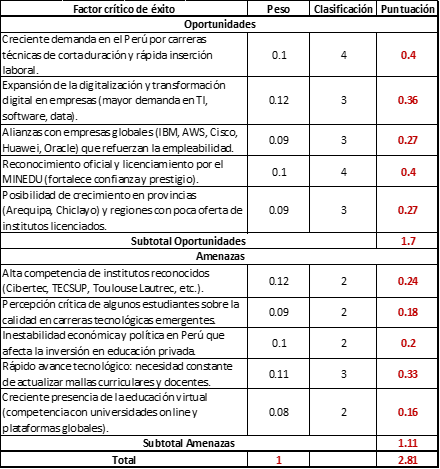
\includegraphics[width=0.8\textwidth]{./assets/matrizEFE.png}
\end{center}



\end{document}